\documentclass[12pt,letterpaper]{article}
\usepackage[latin1]{inputenc}
\usepackage{amsmath}
\usepackage{amsfonts}
\usepackage{amssymb}
\usepackage{graphicx}

\title{CelleratorML Description}
\author{B.E.Shapiro\\Specification Version 1.0.5 {\footnote {Corresponding to CelleratorML.m with the same version number.}}}
\begin{document}

\maketitle
\tableofcontents

\setlength{\parindent}{0pt}
\section{Overview}

This document provides a proposed syntax for CelleratorML.  CelleratorML provides a way of storing Cellerator Models, including initial conditions and parameter values, as ASCII text files, using XML. It is anticipated that future version will include compatibility with the Discrete Grammar sytax proposed by Mjolsness. \\

All Cellerator reactions are represented in MathML. The entire MathML language is allowed, and in fact, is required, to represent Mathematica expressions. Cellerator identifiers that contain characters in Mathematica's extended character set (ISO8559-1) are represented by their ASCII escape codes (see section \ref{subsection:character}).\\

Section \ref{section:CellzillaML} describes a related file format called CellzillaML, which represents Cellzilla Models in XML. \\

Section \ref{section:xmlexamples} provides several complete examples of CelleratorML. \\

The proposed XML has been implemented in the Cellerator plugin package CelleratorML.m. This package is fully compatible with both Cellerator and xCellerator. Worked examples using CelleratorML for both CelleratorML and CellzillaML are given in section \ref{section:implementation}.

\section{CelleratorML}

\subsection{Skeleton File Description of CelleratorML}

CelleratorML contains two XML elements: a ModelAnnotation section; and a CelleratorModel section. A skeleton model is illustrated below: 

\begin{verbatim}
<CelleratorML Version="1.0">

 <ModelAnnotation>
  ... annotation information
 </ModelAnnotation>

 <CelleratorModel name="modelname">

   <ListOfCelleratorReactions>
     ... list of reactions ...
   </ListOfCelleratorReactions>
  
   <ListOfCelleratorParameters>
     ... list of parameters ...
   </ListOfCelleratorParameters>

   <ListOfCelleratorIC>
     ... list of initial conditions ...
   </ListOfCelleratorIC>

 </CelleratorModel>
</CelleratorML>

\end{verbatim}


\subsection{MathML in CelleratorML}
All Cellerator reactions are represented by their MathML functional version version. This way the exact arrow used in the Mathematica notebook is retained upon reloading into Mathematica. For example, a subscripted variable
$$k_F$$
in Mathematica is represented in FullForm as 
$$\text{Subscript}[\text{k}, \text{F}]$$
and the corresponding MathML code segment is
\begin{verbatim}
   <apply>
    <ci>Subscript</ci>
    <ci>k</ci>
    <ci>F</ci>
   </apply>
\end{verbatim}
Since Mathematica implements the entire MathML language, there are no restrictions on which parts of MathML are allowed. 
See section \ref{section:reactions} for an example of a Cellerator arrow in CelleratorML.
\subsection{Identifiers in CelleratorML}\label{subsection:character}
Since Mathematica uses an extended character set not all identifiers can be represented as normal ASCII. To allow use of the extended character set, extended characters are encoded by character codes in ISO8859-1. To find the corresponding character code in use the Mathematica function ToCharacterCode. For example, since the codes of $\alpha$, $\beta$, and $\kappa$ are 945, 946, and 954, respectively, the reaction
$$\{\alpha \rightarrow \beta, \kappa\}$$
becomes
\begin{verbatim}
  <list>
   <apply>
    <ci>ShortRightArrow</ci>
    <ci>&#945;</ci>
    <ci>&#946;</ci>
   </apply>
   <ci>&#954;</ci>
  </list>
\end{verbatim}

\subsection{The $<$ModelAnnotation$>$ object}\label{section:Ann}

The model annotation section contains a place for the program to automatically add identifying information. The reason for including this information, particularly the version numbers, is that sometimes the XML handling functions varies between different version of Mathematica and a program might require this information. \\

The Creator, Email, WebPage and Description fields are optional. The Description field can be either in ASCII text or in html. The CelleratorML.m package automatically adds the CreationTime, MathematicaVersion, MathematicaVersionNumber, MathematicaReleaseNumber, OperatingSystem, and CharacterEncoding fields.\\

The CharacaterEncoding field is the value of the  the Mathematica predefined constant \$CharacterEncoding. The default value of this is ISO8859-1, which is what is used by Mathematica normally. This tells a non-mathematica users that the escape codes in identifiers in other parts of the file are expressed as ISO 8859-1 characters.\\

MathematicaVersion is the value of the Mathematica predefined constant \$Version.\\

MathematicaVersionNumber is the value of the Mathematica predefined constant \$VersionNumber.\\

MathematicaReleaseNumber is the value of the Mathematica predefined constant \$ReleaseNumber.\\

OperatingSystem is the value of the Mathematica predefined constant \$OperatingSystem.\\

\begin{verbatim}
 <ModelAnnotation>
  <CreationTime>2008-11-02T17:52:44</CreationTime>
  <MathematicaVersion>
    6.0 for Linux x86 (32-bit) (June 2, 2008)
  </MathematicaVersion>
  <MathematicaVersionNumber>6.</MathematicaVersionNumber>
  <MathematicaReleaseNumber>3</MathematicaReleaseNumber>
  <OperatingSystem>Linux x86 (32-bit)</OperatingSystem>
  <CharacterEncoding>ISO8859-1</CharacterEncoding>
  <Creator>Joe The Plumber</Creator>
  <Email>joe@the.plumber.com</Email>
  <WebPage>http://www.joetheplumber.com</WebPage>
  <Description>
   <Text>CelleratorML file for faucet repair, by Joe the Plumber</Text>
  </Description>
 </ModelAnnotation>
\end{verbatim}
\$OperatingSystem

\subsection{The $<$CelleratorModel$>$ object}
The CelleratorModel object contains a list of cellerator reactions, parameters, and identifiers. The optional model name tag can be used to specify a model name variable for simulators to used, and hence it can contain any valid Mathematica operator, with extended characters specified with their ASCII character code. 


\begin{verbatim}
 <CelleratorModel name="modelname">

   <ListOfCelleratorReactions>
     ... list of reactions ...
   </ListOfCelleratorReactions>
  
   <ListOfCelleratorParameters>
     ... list of parameters ...
   </ListOfCelleratorParameters>

   <ListOfCelleratorIC>
     ... list of initial conditions ...
   </ListOfCelleratorIC>

 </CelleratorModel>
\end{verbatim}

\subsubsection{The $<$ListOfCelleratorReactions$>$}\label{section:reactions}
The required ListOfCelleratorReactions contains one or more CelleratorReaction assignments. For example, the 
cellerator reaction 
$$\{\text{a} \to \text{b}, \text{k}\}$$
is represented in MathML as:

\begin{verbatim}
<CelleratorReaction>
 <math xmlns='http://www.w3.org/1998/Math/MathML'>
  <list>
   <apply>
    <ci>Rule</ci>
    <ci>a</ci>
    <ci>b</ci>
   </apply>
   <ci>k</ci>
  </list>
 </math>
</CelleratorReaction>
\end{verbatim}
Virtually any Cellerator Reaction can be handled this way. For example, the reaction

$$\left\{\overset{\text{catalyst}}{A\rightleftarrows B},k_1,k_2,k_3\right\}$$
becomes\\

\begin{verbatim}
<CelleratorReaction>
 <math xmlns='http://www.w3.org/1998/Math/MathML'>
  <list>
   <apply>
    <ci>Overscript</ci>
    <apply>
     <ci>RightArrowLeftArrow</ci>
     <ci>A</ci>
     <ci>B</ci>
    </apply>
    <ci>catalyst</ci>
   </apply>
   <apply>
    <ci>Subscript</ci>
    <ci>k</ci>
    <cn type='integer'>1</cn>
   </apply>
   <apply>
    <ci>Subscript</ci>
    <ci>k</ci>
    <cn type='integer'>2</cn>
   </apply>
   <apply>
    <ci>Subscript</ci>
    <ci>k</ci>
    <cn type='integer'>3</cn>
   </apply>
  </list>
 </math>
</CelleratorReaction>
\end{verbatim}
Subscripts, arrows, etc. are all represented in MathML by the Mathematica FullForm Function name.\\

\subsubsection{The $<$ListOfCelleratorParameters$>$}
The required ListOfCelleratorParameters contains zero or more parameter value assignments: 

\begin{verbatim}
   <Parameter 
       Identifier='r1'
       Value='1.' 
       />
\end{verbatim}
means that the parameter r1 has a value of 1. \\

If no parameters are assigned any values in the model then the file should still contain the line
\begin{verbatim}
  <ListOfCelleratorParameters/>
\end{verbatim}


\subsubsection{The $<$ListOfCelleratorIC$>$}\$OperatingSystem
The required ListOfCelleratorIC contains zero or more InitialValue objects:

\begin{verbatim}
   <InitialValue 
       Identifier='AuxIAAProtein'
       Value='0.01' 
      />\$OperatingSystem\$OperatingSystem
\end{verbatim}
means that the species AuxIAAProtein starts with an initial value of 0.01.\\

If there are no Initial Values then the file should still contain the line:

\begin{verbatim}
  <ListOfCelleratorIC />
\end{verbatim}

\section{CellzillaML}\label{section:CellzillaML}

\subsection{Skeleton File Description of CellzillaML}

A CellzillaML file has the following structure: 

\begin{verbatim}
<CellzillaML Version="1.0">
  <ModelAnnotation> .. </ModelAnnotation>
  <CellzillaModel>
    <ListOfCelleratorModels> .. </ListOfCelleratorModels>
    <ListOfDiffusingSpecies> .. </ListOfDiffusingSpecies>
    <ListOfCellzillaParameters> .. </ListOfCellzillaParameters>
    <Centers> .. </Centers>
    <Tissue> .. </Tissue>
    <ListOfCellzillaIC> ..</ListOfCellzillaIC>
  </CellzillaModel>
</CellzillML>
\end{verbatim}

The {\ttfamily $<$ModelAnnotation$>$} has the same structure as the {\ttfamily $<$ModelAnnotation$>$} in CelleratorML as described in section \ref{section:Ann}. The objects within the {\ttfamily $<$CellzillaModel$>$} section are described in the following subsection. 
The order of the objects within the {\ttfamily $<$CellzillaModel$>$} is not significant.\\

Either the {\ttfamily $<$Centers$>$} or the {\ttfamily $<$Tissue$>$} is required. It is not necessary to have both. If only the {\ttfamily $<$Centers$>$} is present it is interpreted by both {\ttfamily Cellzilla} and {\ttfamily Cellzilla2D} as Voronoi Centers for the cells. If the {\ttfamily $<$Tissue$>$}  is present then the {\ttfamily $<$Centers$>$} is not necessary and may be used to represent whatever information the user desires, e.g., cell nuclear centroids. No consistency checks are made to verify that the data in both are consistent, e.g., that there are the same number of centers and cells. If the {\ttfamily Tissue} object is used, then the cell centers are typically ignored. This may change in future versions of {\ttfamily Cellzilla}. 

\subsection{The $<$CellzillaModel$>$}
\subsubsection{The $<$ListOfCelleratorModels$>$}

The $<$ListOfCelleratorModels$>$ contains a list of references to models in CelleratorML. At least one model must be specified. The files are specified either by file name or URL.\\

All of the models are merged together into a single circuit. Any species or parameters that have the same name in different models are assumed to refer to the same species. Initial conditions in the individual models are ignored. Paramater values in the individual models are assumed to be  superceded by any values listed in the $<$ListofCellzillaParameters$>$, although if a parameter value is not listed in the $<$ListOfCellzillaParameters$>$, then the value given in the individual model should be applied. The format is as given in the following example:

\begin{verbatim}
  <ListOfCelleratorModels>
   <CelleratorModel>Wus.xml</CelleratorModel>
   <CelleratorModel>http://my.website.com//myfile.xml</CelleratorModel>
  </ListOfCelleratorModels>
\end{verbatim}

Since file directory name formats vary between operating systems care should be taken in expressing directory names because the model may not be transferable. 


\subsubsection{The $<$ListOfDiffusingSpecies$>$}

Example:
\begin{verbatim}
  <ListOfDiffusingSpecies>
   <DiffusingSpecies Identifier='Y' Rate='Dy' />
   <DiffusingSpecies Identifier='A' Rate='Da' />
   <DiffusingSpecies Identifier='B' Rate='Db' />
  </ListOfDiffusingSpecies>
\end{verbatim}


\subsubsection{The $<$ListOfCellzillaParameters$>$}

Example:
\begin{verbatim}
 <ListOfCellzillaParameters>
   <Parameter Identifier='ky' Value='0.2' />
   <Parameter Identifier='dy' Value='0.1' />
   <Parameter Identifier='Dy' Value='0.1' />
   <Parameter Identifier='kD' Value='3.' />
</ListOfCellzillaParameters>
\end{verbatim}



\subsubsection{The $<$ListOfCellzillaIC$>$}

The {\ttfamily $<$ListOfCellzillaIC$>$} contains a sequence of sub-elements each of which is called a {\ttfamily $<$CellzillaIC$>$}. Each {\ttfamily $<$CellzillaIC$>$} contains one attribute {\ttfamily``Identifier''}, that gives the name of a variable;  and a {\ttfamily ``math''} field, that contains a list of initial values expressed in MathML.

For example, suppose you have two species A and B, in each of 5 cells. To set the initial values to
$A_1=1, A_2=5, A_3=7, A_4=3, A_5=2$ and $B_1=.6, B_2=0, B_3=0, B_4=1, B_5=0$, where $A_i$ or $B_i$ refers to the value of $A$ or $B$ in cell $i$, 

\begin{verbatim}
<ListOfCellzillaIC>
 <CellzillaIC Identifier='A'>
  <math xmlns='http://www.w3.org/1998/Math/MathML'>
   <list>
    <cn type='real'>1.</cn>
    <cn type='real'>5.</cn>
    <cn type='real'>7.</cn>
    <cn type='real'>3.</cn>
    <cn type='real'>2.</cn>
   </list>
  </math>
 </CellzillaIC>
 <CellzillaIC Identifier='B'>
  <math xmlns='http://www.w3.org/1998/Math/MathML'>
   <list>
    <cn type='real'>0.6</cn>
    <cn type='real'>0.</cn>
    <cn type='real'>0.</cn>
    <cn type='real'>1.</cn>
    <cn type='real'>0.</cn>
   </list>
  </math>
 </CellzillaIC>
</ListOfCellzillaIC>
\end{verbatim}

\subsubsection{The $<$Centers$>$}
Centers contains a list of lists expressed in MathML. Each sublist should 
have dimension equal to the value of the attribute {\ttfamily ``Dimension''}. Only dimension 2 is currently supported by Cellzilla.\\

Example:
\begin{verbatim}
  <Centers Dimension='2'>
   <math xmlns='http://www.w3.org/1998/Math/MathML'>
    <list>
     <list>
      <cn type='real'>10.294969120832743</cn>
      <cn type='real'>29.28472172065968</cn>
     </list>
     <list>
      <cn type='real'>19.7677222064611</cn>
      <cn type='real'>27.34192006467375</cn>
     </list>
     ...
     <list>
      <cn type='real'>78.84929650925012</cn>
      <cn type='real'>53.881100791258405</cn>
     </list>
    </list>
   </math>
  </Centers>
\end{verbatim}

\subsubsection{The $<$Tissue$>$}

This contains the Cellzilla2D tissue object; Tissue objects are not processed by Cellzilla, but only by Cellzilla2D. \\

There are three parts: The Vertices, Edges, and Cells.  In 3D (not implemented) there are four parts: The Vertices, Edges, Faces, and Cells.\\

The vertices contains a list of vertex coordinates. The Dimension of each coordinate pair must be the same as the tissue dimension. Only Dimension=2 is implemented currently. Each coordinate pair is a list representing x and y coordinates. The order of vertices is crucial since they will be referenced by their position in this list by the edges.\\

The edges contain a list of edge pairs. Each edge pair is a pair of integers represented by a list. The two integers represent vertices. For example, if the edge contains the integers $\{23, 5\}$ then there is an edge between the 23$^{rd}$ and 5$^{th}$ vertex in the list of vertices. The order of the edges is crucial since they will be referenced by their position in the edge list by teh cells list.\\

The cells list contains a list of lists. Each list represents one cell, and is a list of integers. The integers represent edges of the cell. For example, if a cell is $\{4, 7, 9, 13, 23\}$ then the cell's edges are reprsented by the edges in position 4, 7, 9, 13, and 23 of the list of edges. \\


Example:
\begin{verbatim}
 <Tissue Dimension='2'>
   <Vertices Dimension='2'>
    <math xmlns='http://www.w3.org/1998/Math/MathML'>
     <list>
      <list>
       <cn type='real'>-15.148929333300346</cn>
       <cn type='real'>17.932819513551138</cn>
      </list>
      <list>
     ...
    </math>
   </Vertices>
   <Edges>
    <math xmlns='http://www.w3.org/1998/Math/MathML'>
     <list>
      <list>
       <cn type='integer'>1</cn>
       <cn type='integer'>2</cn>
      </list>
      <list>     
      ...
     </math>
   </Edges>
   <Cells>
    <math xmlns='http://www.w3.org/1998/Math/MathML'>
     <list>
      <list>
       <cn type='integer'>2</cn>
       <cn type='integer'>1</cn>
       <cn type='integer'>3</cn>
       <cn type='integer'>14</cn>
       <cn type='integer'>15</cn>
       <cn type='integer'>17</cn>
       <cn type='integer'>11</cn>
       <cn type='integer'>4</cn>
      </list>
      ...
   </Cells>
  </Tissue>
\end{verbatim}


\section{XML Examples}\label{section:xmlexamples}

\subsection{CelleratorML Example}

Consider the simple toy Cellerator model

$$\left\{\left\{\alpha \rightleftarrows \beta
   ,k_f,k_r\right\},\left\{\emptyset \rightarrow \alpha
   ,k_1\right\},\left\{\beta \to \alpha ,k_2\right\}\right\}$$
with all rate constants set to 1 and all initial conditions set to zero. Then the CelleratorML is: 

\begin{verbatim}
<?xml version='1.0' encoding='ASCII'?>
<!-- Generated 02 November 2008 at 18:30 GMT-07:60 -->
<!-- Generated by CelleratorML 0.1 (31 Oct 2008) -->
<!-- Generated using Mathematica Version 6.0 for Linux x86 (32-bit) 
     (June 2, 2008) (Release 3)-->
<CelleratorML Version='1.0'>
 <ModelAnnotation>
  <CreationTime>2008-11-02T18:30:00</CreationTime>
  <MathematicaVersion>
   6.0 for Linux x86 (32-bit) (June 2, 2008)
  </MathematicaVersion>
  <MathematicaVersionNumber>6.</MathematicaVersionNumber>
  <MathematicaReleaseNumber>3</MathematicaReleaseNumber>
  <OperatingSystem>Linux x86 (32-bit)</OperatingSystem>
  <CharacterEncoding>ISO8859-1</CharacterEncoding>
  <Creator>mathman</Creator>
  <Description>
   <html>This is a CelleratorML (XML) file.</html>
  </Description>
 </ModelAnnotation>
 <CelleratorModel Name='Model2'>
  <ListOfCelleratorReactions>
   <CelleratorReaction>
    <math xmlns='http://www.w3.org/1998/Math/MathML'>
     <list>
      <apply>
       <ci>RightArrowLeftArrow</ci>
       <ci>&#945;</ci>
       <ci>&#946;</ci>
      </apply>
      <apply>
       <ci>Subscript</ci>
       <ci>k</ci>
       <ci>f</ci>
      </apply>
      <apply>
       <ci>Subscript</ci>
       <ci>k</ci>
       <ci>r</ci>
      </apply>
     </list>
    </math>
   </CelleratorReaction>
   <CelleratorReaction>
    <math xmlns='http://www.w3.org/1998/Math/MathML'>
     <list>
      <apply>
       <ci>ShortRightArrow</ci>
       <ci>&#8709;</ci>
       <ci>&#945;</ci>
      </apply>
      <apply>
       <ci>Subscript</ci>
       <ci>k</ci>
       <cn type='integer'>1</cn>
      </apply>
     </list>
    </math>
   </CelleratorReaction>
   <CelleratorReaction>
    <math xmlns='http://www.w3.org/1998/Math/MathML'>
     <list>
      <apply>
       <ci>Rule</ci>
       <ci>&#946;</ci>
       <ci>&#945;</ci>
      </apply>
      <apply>
       <ci>Subscript</ci>
       <ci>k</ci>
       <cn type='integer'>2</cn>
      </apply>
     </list>
    </math>
   </CelleratorReaction>
  </ListOfCelleratorReactions>
  <ListOfCelleratorParameters>
   <Parameter Identifier='k' Value='1' />
   <Parameter Identifier='Subscript[k, f]' Value='1' />
   <Parameter Identifier='Subscript[k, r]' Value='1' />
   <Parameter Identifier='Subscript[k, 1]' Value='1' />
   <Parameter Identifier='Subscript[k, 2]' Value='1' />
  </ListOfCelleratorParameters>
  <ListOfCelleratorIC>
   <InitialValue Identifier='&#945;' Value='0' />
   <InitialValue Identifier='&#946;' Value='0' />
  </ListOfCelleratorIC>
 </CelleratorModel>
</CelleratorML>
\end{verbatim}

\subsection{CelleratorML for Oscillations in MAPK}

Consider the following Cellerator model of MAPK Oscillations (based on Kholodenko's model) (the \LaTeX was typeset with the CelleratorML.m function LatexForm): 


$$\{\emptyset \rightleftarrows S,\text{a0},\text{d0}\}$$
$$\left\{\overset{S}{\text{KKK}\rightleftarrows \text{KKKp}},\{\text{a1},\text{d1},\text{k1}\}\right\}$$
$$\left\{\overset{\text{KKKp}}{\text{KK}\rightleftarrows \text{KKp}},\{\text{a3},\text{d3},\text{k3}\}\right\}$$
$$\left\{\overset{\text{KKKp}}{\text{KKp}\rightleftarrows \text{KKpp}},\{\text{a3},\text{d3},\text{k3}\}\right\}$$
$$\left\{\overset{\text{KKpp}}{\text{MAPK}\rightleftarrows \text{Kp}},\{\text{a3},\text{d3},\text{k3}\}\right\}$$
$$\left\{\overset{\text{KKpp}}{\text{Kp}\rightleftarrows \text{Kpp}},\{\text{a3},\text{d3},\text{k3}\}\right\}$$
$$\{\text{Kpp}+\text{Bind}(\text{KKK},S)\rightleftarrows \text{KKK$\$$S$\$$Kpp},\text{a7},\text{d7}\}$$
$$\left\{\overset{\text{KKKph}}{\text{KKKp}\rightleftarrows \text{KKK}},\{\text{a4},\text{d4},\text{k4}\}\right\}$$
$$\left\{\overset{\text{KKph}}{\text{KKp}\rightleftarrows \text{KK}},\{\text{a5},\text{d5},\text{k5}\}\right\}$$
$$\left\{\overset{\text{KKph}}{\text{KKpp}\rightleftarrows \text{KKp}},\{\text{a5},\text{d5},\text{k5}\}\right\}$$
$$\left\{\overset{\text{Kph}}{\text{Kpp}\rightleftarrows \text{Kp}},\{\text{a6},\text{d6},\text{k6}\}\right\}$$
$$\left\{\overset{\text{Kph}}{\text{Kp}\rightleftarrows \text{MAPK}},\{\text{a6},\text{d6},\text{k6}\}\right\}$$
with initial conditions  $\text{KKK}=100$,
$\text{KKKp}=0$,
$\text{KK}=300$,
$\text{KKp}=0$,
$\text{KKpp}=0$,
$\text{MAPK}=300$,
$\text{Kp}=0$,
$\text{Kpp}=0$,
$S=1$,
$\text{Kph}=1$,
$\text{KKph}=1$,
$\text{KKKph}=10$ and parameter values $\text{a0}=1$,
$\text{d0}=1$,
$\text{a1}=1$,
$\text{d1}=7.5$,
$\text{k1}=2.5$,
$\text{a3}=1$,
$\text{d3}=10$,
$\text{k3}=0.025$,
$\text{a4}=1$,
$\text{d4}=1$,
$\text{k4}=1$,
$\text{a5}=1$,
$\text{d5}=1$,
$\text{k5}=1$,
$\text{a6}=1$,
$\text{d6}=1$,
$\text{k6}=1$,
$\text{a7}=1$,
$\text{d7}=1$.

The CelleratorML (which can be automatically generated from the model by the CelleratorML.m function SaveModel), is shown below.

\begin{verbatim}
<?xml version='1.0' encoding='ASCII'?>
<!-- Generated 02 November 2008 at 18:08 GMT-07:60 -->
<!-- Generated by CelleratorML 0.1 (31 Oct 2008) -->
<!-- Generated using Mathematica Version 6.0 for Linux x86 (32-bit)
(June 2, 2008) (Release 3)-->
<CelleratorML Version='1.0'>
 <ModelAnnotation>
  <CreationTime>2008-11-02T18:08:32</CreationTime>
  <MathematicaVersion>
    6.0 for Linux x86 (32-bit) (June 2, 2008)
  </MathematicaVersion>
  <MathematicaVersionNumber>6.</MathematicaVersionNumber>
  <MathematicaReleaseNumber>3</MathematicaReleaseNumber>
  <OperatingSystem>Linux x86 (32-bit)</OperatingSystem>
  <CharacterEncoding>ISO8859-1</CharacterEncoding>
  <Creator>mathman</Creator>
  <Description>
   <html>This is a CelleratorML (XML) file.</html>
  </Description>
 </ModelAnnotation>
 <CelleratorModel Name='Model1'>
  <ListOfCelleratorReactions>
   <CelleratorReaction>
    <math xmlns='http://www.w3.org/1998/Math/MathML'>
     <list>
      <apply>
       <ci>RightArrowLeftArrow</ci>
       <ci>&#8709;</ci>
       <ci>S</ci>
      </apply>
      <ci>a0</ci>
      <ci>d0</ci>
     </list>
    </math>
   </CelleratorReaction>
   <CelleratorReaction>
    <math xmlns='http://www.w3.org/1998/Math/MathML'>
     <list>
      <apply>
       <ci>Overscript</ci>
       <apply>
        <ci>RightArrowLeftArrow</ci>
        <ci>KKK</ci>
        <ci>KKKp</ci>
       </apply>
       <ci>S</ci>
      </apply>
      <list>
       <ci>a1</ci>
       <ci>d1</ci>
       <ci>k1</ci>
      </list>
     </list>
    </math>
   </CelleratorReaction>
   <CelleratorReaction>
    <math xmlns='http://www.w3.org/1998/Math/MathML'>
     <list>
      <apply>
       <ci>Overscript</ci>
       <apply>
        <ci>RightArrowLeftArrow</ci>
        <ci>KK</ci>
        <ci>KKp</ci>
       </apply>
       <ci>KKKp</ci>
      </apply>
      <list>
       <ci>a3</ci>
       <ci>d3</ci>
       <ci>k3</ci>
      </list>
     </list>
    </math>
   </CelleratorReaction>
   <CelleratorReaction>
    <math xmlns='http://www.w3.org/1998/Math/MathML'>
     <list>
      <apply>
       <ci>Overscript</ci>
       <apply>
        <ci>RightArrowLeftArrow</ci>
        <ci>KKp</ci>
        <ci>KKpp</ci>
       </apply>
       <ci>KKKp</ci>
      </apply>
      <list>
       <ci>a3</ci>
       <ci>d3</ci>
       <ci>k3</ci>
      </list>
     </list>
    </math>
   </CelleratorReaction>
   <CelleratorReaction>
    <math xmlns='http://www.w3.org/1998/Math/MathML'>
     <list>
      <apply>
       <ci>Overscript</ci>
       <apply>
        <ci>RightArrowLeftArrow</ci>
        <ci>MAPK</ci>
        <ci>Kp</ci>
       </apply>
       <ci>KKpp</ci>
      </apply>
      <list>
       <ci>a3</ci>
       <ci>d3</ci>
       <ci>k3</ci>
      </list>
     </list>
    </math>
   </CelleratorReaction>
   <CelleratorReaction>
    <math xmlns='http://www.w3.org/1998/Math/MathML'>
     <list>
      <apply>
       <ci>Overscript</ci>
       <apply>
        <ci>RightArrowLeftArrow</ci>
        <ci>Kp</ci>
        <ci>Kpp</ci>
       </apply>
       <ci>KKpp</ci>
      </apply>
      <list>
       <ci>a3</ci>
       <ci>d3</ci>
       <ci>k3</ci>
      </list>
     </list>
    </math>
   </CelleratorReaction>
   <CelleratorReaction>
    <math xmlns='http://www.w3.org/1998/Math/MathML'>
     <list>
      <apply>
       <ci>RightArrowLeftArrow</ci>
       <apply>
        <plus />
        <ci>Kpp</ci>
        <apply>
         <ci>Bind</ci>
         <ci>KKK</ci>
         <ci>S</ci>
        </apply>
       </apply>
       <ci>KKK$S$Kpp</ci>
      </apply>
      <ci>a7</ci>
      <ci>d7</ci>
     </list>
    </math>
   </CelleratorReaction>
   <CelleratorReaction>
    <math xmlns='http://www.w3.org/1998/Math/MathML'>
     <list>
      <apply>
       <ci>Overscript</ci>
       <apply>
        <ci>RightArrowLeftArrow</ci>
        <ci>KKKp</ci>
        <ci>KKK</ci>
       </apply>
       <ci>KKKph</ci>
      </apply>
      <list>
       <ci>a4</ci>
       <ci>d4</ci>
       <ci>k4</ci>
      </list>
     </list>
    </math>
   </CelleratorReaction>
   <CelleratorReaction>
    <math xmlns='http://www.w3.org/1998/Math/MathML'>
     <list>
      <apply>
       <ci>Overscript</ci>
       <apply>
        <ci>RightArrowLeftArrow</ci>
        <ci>KKp</ci>
        <ci>KK</ci>
       </apply>
       <ci>KKph</ci>
      </apply>
      <list>
       <ci>a5</ci>
       <ci>d5</ci>
       <ci>k5</ci>
      </list>
     </list>
    </math>
   </CelleratorReaction>
   <CelleratorReaction>
    <math xmlns='http://www.w3.org/1998/Math/MathML'>
     <list>
      <apply>
       <ci>Overscript</ci>
       <apply>
        <ci>RightArrowLeftArrow</ci>
        <ci>KKpp</ci>
        <ci>KKp</ci>
       </apply>
       <ci>KKph</ci>
      </apply>
      <list>
       <ci>a5</ci>
       <ci>d5</ci>
       <ci>k5</ci>
      </list>
     </list>
    </math>
   </CelleratorReaction>
   <CelleratorReaction>
    <math xmlns='http://www.w3.org/1998/Math/MathML'>
     <list>
      <apply>
       <ci>Overscript</ci>
       <apply>
        <ci>RightArrowLeftArrow</ci>
        <ci>Kpp</ci>
        <ci>Kp</ci>
       </apply>
       <ci>Kph</ci>
      </apply>
      <list>
       <ci>a6</ci>
       <ci>d6</ci>
       <ci>k6</ci>
      </list>
     </list>
    </math>
   </CelleratorReaction>
   <CelleratorReaction>
    <math xmlns='http://www.w3.org/1998/Math/MathML'>
     <list>
      <apply>
       <ci>Overscript</ci>
       <apply>
        <ci>RightArrowLeftArrow</ci>
        <ci>Kp</ci>
        <ci>MAPK</ci>
       </apply>
       <ci>Kph</ci>
      </apply>
      <list>
       <ci>a6</ci>
       <ci>d6</ci>
       <ci>k6</ci>
      </list>
     </list>
    </math>
   </CelleratorReaction>
  </ListOfCelleratorReactions>
  <ListOfCelleratorParameters>
   <Parameter Identifier='a0' Value='1' />
   <Parameter Identifier='d0' Value='1' />
   <Parameter Identifier='a1' Value='1' />
   <Parameter Identifier='d1' Value='7.5' />
   <Parameter Identifier='k1' Value='2.5' />
   <Parameter Identifier='a3' Value='1' />
   <Parameter Identifier='d3' Value='10' />
   <Parameter Identifier='k3' Value='0.025' />
   <Parameter Identifier='a4' Value='1' />
   <Parameter Identifier='d4' Value='1' />
   <Parameter Identifier='k4' Value='1' />
   <Parameter Identifier='a5' Value='1' />
   <Parameter Identifier='d5' Value='1' />
   <Parameter Identifier='k5' Value='1' />
   <Parameter Identifier='a6' Value='1' />
   <Parameter Identifier='d6' Value='1' />
   <Parameter Identifier='k6' Value='1' />
   <Parameter Identifier='a7' Value='1' />
   <Parameter Identifier='d7' Value='1' />
  </ListOfCelleratorParameters>
  <ListOfCelleratorIC>
   <InitialValue Identifier='KKK'   Value='100' />
   <InitialValue Identifier='KKKp'  Value='0' />
   <InitialValue Identifier='KK'    Value='300' />
   <InitialValue Identifier='KKp'   Value='0' />
   <InitialValue Identifier='KKpp'  Value='0' />
   <InitialValue Identifier='MAPK'  Value='300' />
   <InitialValue Identifier='Kp'    Value='0' />
   <InitialValue Identifier='Kpp'   Value='0' />
   <InitialValue Identifier='S'     Value='1' />
   <InitialValue Identifier='Kph'   Value='1' />
   <InitialValue Identifier='KKph'  Value='1' />
   <InitialValue Identifier='KKKph' Value='10' />
  </ListOfCelleratorIC>
 </CelleratorModel>
</CelleratorML>
\end{verbatim}

\subsection{Wuschel Model in a Single Cell}

The following model implements the Wuschel model described in [Jonsson et al (2005) Bioinformatics 21(S1):i232-i240]. The cellerator reactions for the model are:
$$\left\{Y\mapsto W,\text{GRN}\left(\frac{1}{\text{tauw}},\text{Twy},1,\text{hw},\sigma \right)\right\}$$
$$\left\{A\mapsto W,\text{GRN}\left(\frac{1}{\text{tauw}},\text{Twa},1,\text{hw},\sigma \right)\right\}$$
$$\{W\rightarrow \emptyset ,\text{dw}\}$$
$$\{\text{L1}\rightarrow \text{L1}+Y,\text{ky}\}$$
$$\{Y\rightarrow \emptyset ,\text{dy}\}$$
$$\{A+Y\rightarrow Y,d\}$$
$$\{\emptyset \rightleftarrows A,a,\beta \}$$
$$\{2 A+B\rightarrow 3 A,c\}$$
$$\{A\rightarrow B,b\}$$
 Parameter values and Initial conditions are not specified in this example.

\begin{verbatim}
<?xml version='1.0' encoding='ASCII'?>
<!-- Generated 30 November 2008 at 12:54 GMT-07:60 -->
<!-- Generated by CelleratorML 1.0.3 (30 Nov 2008) -->
<!-- Generated using Mathematica Version 7.0 for Linux x86 
     (32-bit) (November 11, 2008) (Release 0)-->
<CelleratorML Version='1.0'>
 <ModelAnnotation>
  <CreationTime>2008-11-30T12:54:13</CreationTime>
  <MathematicaVersion>7.0 for Linux x86 (32-bit) 
  (November 11, 2008)</MathematicaVersion>
  <MathematicaVersionNumber>7.</MathematicaVersionNumber>
  <MathematicaReleaseNumber>0</MathematicaReleaseNumber>
  <OperatingSystem>Linux x86 (32-bit)</OperatingSystem>
  <CharacterEncoding>ISO8859-1</CharacterEncoding>
  <Creator>mathman</Creator>
  <Description>
   <html>This is a CelleratorML (XML) file.</html>
  </Description>
 </ModelAnnotation>
 <CelleratorModel Name='Model1'>
  <ListOfCelleratorReactions>
   <CelleratorReaction>
    <math xmlns='http://www.w3.org/1998/Math/MathML'>
     <list>
      <apply>
       <ci>RightTeeArrow</ci>
       <ci>Y</ci>
       <ci>W</ci>
      </apply>
      <apply>
       <ci>GRN</ci>
       <apply>
        <times />
        <cn type='integer'>1</cn>
        <apply>
         <power />
         <ci>tauw</ci>
         <cn type='integer'>-1</cn>
        </apply>
       </apply>
       <ci>Twy</ci>
       <cn type='integer'>1</cn>
       <ci>hw</ci>
       <ci>sigma</ci>
      </apply>
     </list>
    </math>
   </CelleratorReaction>
   <CelleratorReaction>
    <math xmlns='http://www.w3.org/1998/Math/MathML'>
     <list>
      <apply>
       <ci>RightTeeArrow</ci>
       <ci>A</ci>
       <ci>W</ci>
      </apply>
      <apply>
       <ci>GRN</ci>
       <apply>
        <times />
        <cn type='integer'>1</cn>
        <apply>
         <power />
         <ci>tauw</ci>
         <cn type='integer'>-1</cn>
        </apply>
       </apply>
       <ci>Twa</ci>
       <cn type='integer'>1</cn>
       <ci>hw</ci>
       <ci>sigma</ci>
      </apply>
     </list>
    </math>
   </CelleratorReaction>
   <CelleratorReaction>
    <math xmlns='http://www.w3.org/1998/Math/MathML'>
     <list>
      <apply>
       <ci>ShortRightArrow</ci>
       <ci>W</ci>
       <ci>&#8709;</ci>
      </apply>
      <ci>dw</ci>
     </list>
    </math>
   </CelleratorReaction>
   <CelleratorReaction>
    <math xmlns='http://www.w3.org/1998/Math/MathML'>
     <list>
      <apply>
       <ci>ShortRightArrow</ci>
       <ci>L1</ci>
       <apply>
        <plus />
        <ci>L1</ci>
        <ci>Y</ci>
       </apply>
      </apply>
      <ci>ky</ci>
     </list>
    </math>
   </CelleratorReaction>
   <CelleratorReaction>
    <math xmlns='http://www.w3.org/1998/Math/MathML'>
     <list>
      <apply>
       <ci>ShortRightArrow</ci>
       <ci>Y</ci>
       <ci>&#8709;</ci>
      </apply>
      <ci>dy</ci>
     </list>
    </math>
   </CelleratorReaction>
   <CelleratorReaction>
    <math xmlns='http://www.w3.org/1998/Math/MathML'>
     <list>
      <apply>
       <ci>ShortRightArrow</ci>
       <apply>
        <plus />
        <ci>A</ci>
        <ci>Y</ci>
       </apply>
       <ci>Y</ci>
      </apply>
      <ci>d</ci>
     </list>
    </math>
   </CelleratorReaction>
   <CelleratorReaction>
    <math xmlns='http://www.w3.org/1998/Math/MathML'>
     <list>
      <apply>
       <ci>RightArrowLeftArrow</ci>
       <ci>&#8709;</ci>
       <ci>A</ci>
      </apply>
      <ci>a</ci>
      <ci>beta</ci>
     </list>
    </math>
   </CelleratorReaction>
   <CelleratorReaction>
    <math xmlns='http://www.w3.org/1998/Math/MathML'>
     <list>
      <apply>
       <ci>ShortRightArrow</ci>
       <apply>
        <plus />
        <apply>
         <times />
         <cn type='integer'>2</cn>
         <ci>A</ci>
        </apply>
        <ci>B</ci>
       </apply>
       <apply>
        <times />
        <cn type='integer'>3</cn>
        <ci>A</ci>
       </apply>
      </apply>
      <ci>c</ci>
     </list>
    </math>
   </CelleratorReaction>
   <CelleratorReaction>
    <math xmlns='http://www.w3.org/1998/Math/MathML'>
     <list>
      <apply>
       <ci>ShortRightArrow</ci>
       <ci>A</ci>
       <ci>B</ci>
      </apply>
      <ci>b</ci>
     </list>
    </math>
   </CelleratorReaction>
  </ListOfCelleratorReactions>
  <ListOfCelleratorParameters />
  <ListOfCelleratorIC />
 </CelleratorModel>
</CelleratorML>
\end{verbatim}

\subsection{CellzillaML for Wuschel on a Template}
The Wuschel model will be implemented on the template defined by the following (approximate) cell centers: 
\{\{10.3, 29.3\}, \{19.8, 27.3\}, \{78.8, 53.9\}, \{85.7, 40.4\}, \{34.5, 
  54.9\}, \{0.2, 30.4\}, \{56.4, 71.7\}, \{4.6, 61.8\}, \{22.4, 9.3\}, \{76.5, 
  52.\}, \{1., 10.9\}, \{10.4, 24.7\}\} (rounded to one decimal place) using the following parameter values: with the following parameter values: ky=0.2, dy=0.1, Dy=0.1, kD=3.0, tauw=10, dw=0.1, 
 hw=0, Twy=-20, Twa=0.5, a=0.1, b=0.2, beta=0.1, 
 c=0.1, d=0.01, Da=0.1, Db=1.5. The truncated-voronoi geometry deduced by Cellzilla is illustrated in the following figure. Initial conditions for all species are set to zero, except for L1, which is set to 1 on the boundary cells and to 0 on the interior cells (cells 1 and 12 in the figure).  
  \begin{center}
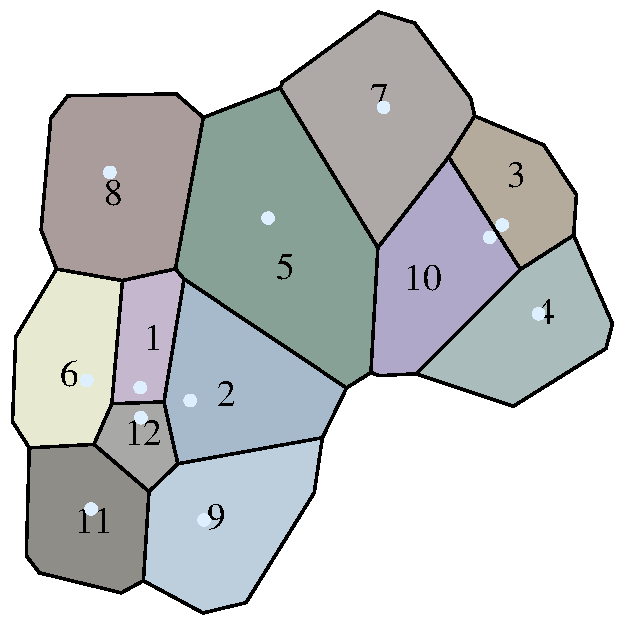
\includegraphics[scale=.7]{template.pdf}
\end{center}

\begin{verbatim}
<?xml version='1.0' encoding='ASCII'?>
<!-- Generated 02 December 2008 at 09:14 GMT-07:60 -->
<!-- Generated by CelleratorML 1.0.3 (30 Nov 2008) -->
<!-- Generated using Mathematica Version 7.0 for Linux x86 (32-bit) 
     (November 11, 2008) (Release 0)-->
<CellzillaML Version='1.0'>
 <ModelAnnotation>
  <CreationTime>2008-12-02T09:14:16</CreationTime>
  <MathematicaVersion>7.0 for Linux x86 (32-bit) 
   (November 11, 2008)</MathematicaVersion>
  <MathematicaVersionNumber>7.</MathematicaVersionNumber>
  <MathematicaReleaseNumber>0</MathematicaReleaseNumber>
  <OperatingSystem>Linux x86 (32-bit)</OperatingSystem>
  <CharacterEncoding>ISO8859-1</CharacterEncoding>
  <Creator>mathman</Creator>
  <Description>
   <Text>This is a CellzillaML (XML) file.</Text>
  </Description>
 </ModelAnnotation>
 <CellzillaModel Name='Wuschel&#9141;Model&#9141;12&#9141;Cells'>
  <ListOfCelleratorModels>
   <CelleratorModel>Wus.xml</CelleratorModel>
  </ListOfCelleratorModels>
  <ListOfDiffusingSpecies>
   <DiffusingSpecies Identifier='Y'Rate='Dy' />
   <DiffusingSpecies Identifier='A' Rate='Da' />
   <DiffusingSpecies Identifier='B' Rate='Db' />
  </ListOfDiffusingSpecies>
  <ListOfCellzillaParameters>
   <Parameter Identifier='ky'Value='0.2' />
   <Parameter Identifier='dy'Value='0.1' />
   <Parameter Identifier='Dy'Value='0.1' />
   <Parameter Identifier='kD'Value='3.' />
   <Parameter Identifier='tauw'Value='10' />
   <Parameter Identifier='dw' Value='0.1' />
   <Parameter Identifier='hw' Value='0' />
   <Parameter Identifier='Twy' Value='-20' />
   <Parameter Identifier='Twa' Value='0.5' />
   <Parameter Identifier='a' Value='0.1' />
   <Parameter Identifier='b' Value='0.2' />
   <Parameter Identifier='beta' Value='0.1' />
   <Parameter Identifier='c' Value='0.1' />
   <Parameter Identifier='d' Value='0.01' />
   <Parameter Identifier='Da' Value='0.1' />
   <Parameter Identifier='Db' Value='1.5' />
  </ListOfCellzillaParameters>
  <Centers Dimension='2'>
   <math xmlns='http://www.w3.org/1998/Math/MathML'>
    <list>
     <list>
      <cn type='real'>10.294969120832743</cn>
      <cn type='real'>29.28472172065968</cn>
     </list>
     <list>
      <cn type='real'>19.7677222064611</cn>
      <cn type='real'>27.34192006467375</cn>
     </list>
     <list>
      <cn type='real'>78.84929650925012</cn>
      <cn type='real'>53.881100791258405</cn>
     </list>
     <list>
      <cn type='real'>85.7460037185621</cn>
      <cn type='real'>40.432209858614286</cn>
     </list>
     <list>
      <cn type='real'>34.51149028352034</cn>
      <cn type='real'>54.91111266903543</cn>
     </list>
     <list>
      <cn type='real'>0.17224206205412873</cn>
      <cn type='real'>30.382759350425538</cn>
     </list>
     <list>
      <cn type='real'>56.40671049004167</cn>
      <cn type='real'>71.67395981256779</cn>
     </list>
     <list>
      <cn type='real'>4.557482566327664</cn>
      <cn type='real'>61.83400948551754</cn>
     </list>
     <list>
      <cn type='real'>22.372074424081</cn>
      <cn type='real'>9.255950931034507</cn>
     </list>
     <list>
      <cn type='real'>76.49967095793389</cn>
      <cn type='real'>52.00127331057238</cn>
     </list>
     <list>
      <cn type='real'>0.9983199916422825</cn>
      <cn type='real'>10.941072213560421</cn>
     </list>
     <list>
      <cn type='real'>10.425342023505602</cn>
      <cn type='real'>24.728856768496964</cn>
     </list>
    </list>
   </math>
  </Centers>
  <ListOfCellzillaIC>
   <CellzillaIC Identifier='A'>
    <math xmlns='http://www.w3.org/1998/Math/MathML'>
     <list>
      <cn type='integer'>0</cn>
      <cn type='integer'>0</cn>
      <cn type='integer'>0</cn>
      <cn type='integer'>0</cn>
      <cn type='integer'>0</cn>
      <cn type='integer'>0</cn>
      <cn type='integer'>0</cn>
      <cn type='integer'>0</cn>
      <cn type='integer'>0</cn>
      <cn type='integer'>0</cn>
      <cn type='integer'>0</cn>
      <cn type='integer'>0</cn>
     </list>
    </math>
   </CellzillaIC>
   <CellzillaIC Identifier='B'>
    <math xmlns='http://www.w3.org/1998/Math/MathML'>
     <list>
      <cn type='integer'>0</cn>
      <cn type='integer'>0</cn>
      <cn type='integer'>0</cn>
      <cn type='integer'>0</cn>
      <cn type='integer'>0</cn>
      <cn type='integer'>0</cn>
      <cn type='integer'>0</cn>
      <cn type='integer'>0</cn>
      <cn type='integer'>0</cn>
      <cn type='integer'>0</cn>
      <cn type='integer'>0</cn>
      <cn type='integer'>0</cn>
     </list>
    </math>
   </CellzillaIC>
   <CellzillaIC Identifier='L1'>
    <math xmlns='http://www.w3.org/1998/Math/MathML'>
     <list>
      <cn type='integer'>0</cn>
      <cn type='integer'>1</cn>
      <cn type='integer'>1</cn>
      <cn type='integer'>1</cn>
      <cn type='integer'>1</cn>
      <cn type='integer'>1</cn>
      <cn type='integer'>1</cn>
      <cn type='integer'>1</cn>
      <cn type='integer'>1</cn>
      <cn type='integer'>1</cn>
      <cn type='integer'>1</cn>
      <cn type='integer'>0</cn>
     </list>
    </math>
   </CellzillaIC>
   <CellzillaIC Identifier='W'>
    <math xmlns='http://www.w3.org/1998/Math/MathML'>
     <list>
      <cn type='integer'>0</cn>
      <cn type='integer'>0</cn>
      <cn type='integer'>0</cn>
      <cn type='integer'>0</cn>
      <cn type='integer'>0</cn>
      <cn type='integer'>0</cn>
      <cn type='integer'>0</cn>
      <cn type='integer'>0</cn>
      <cn type='integer'>0</cn>
      <cn type='integer'>0</cn>
      <cn type='integer'>0</cn>
      <cn type='integer'>0</cn>
     </list>
    </math>
   </CellzillaIC>
   <CellzillaIC Identifier='Y'>
    <math xmlns='http://www.w3.org/1998/Math/MathML'>
     <list>
      <cn type='integer'>0</cn>
      <cn type='integer'>0</cn>
      <cn type='integer'>0</cn>
      <cn type='integer'>0</cn>
      <cn type='integer'>0</cn>
      <cn type='integer'>0</cn>
      <cn type='integer'>0</cn>
      <cn type='integer'>0</cn>
      <cn type='integer'>0</cn>
      <cn type='integer'>0</cn>
      <cn type='integer'>0</cn>
      <cn type='integer'>0</cn>
     </list>
    </math>
   </CellzillaIC>
  </ListOfCellzillaIC>
 </CellzillaModel>
</CellzillaML>
\end{verbatim}

\section{Implementation: CelleratorML.m}\label{section:implementation}




CelleratorML.m is a mathematica packagte that implements both CelleratorML and CellzillaML. The first subsection presents an annotated example of how to use the
package and the second subsection presents list of the functions that are available in the package. 

\subsection{Worked Examples}
\subsubsection{Prerequisites}
The following packages must be installed before using the CelleratorML package.
\begin{itemize}
\item CelleratorML Mathematica Package from http://sf.net/proejcts/xlr8r/
\item xCellerator Mathematica Package from http://sf.net/projects/xlr8r/
\item mPower Mathematica Package from http://sf.net/projects/xlr8r/
\item cellzilla Mathematica Package from http://sf.net/projects/xlr8r/
\item MathSBML Mathematica Package from http://sf.net/projects/SBML/
\item qhull binaries from http://www.qhull.org/
\end{itemize}
CelleratorML works with either Mathematica Version 6.0.3 or 7.0. It has
not been tested on earlier versions. 
\subsubsection{Toy Example: Ring Oscillator}

We consider the ring oscillator based on the following Cellerator Reactions using 
Michaelis-Menten Kinetics: 
$$\left\{\underset{Z_P}{\overset{Z}{X\Longleftrightarrow {X_P}}},\text{MM}(K,v,K,v)\right\}$$
$$\left\{\underset{X_P}{\overset{X}{Y\Longleftrightarrow {Y_P}}},\text{MM}(K,v,K,v)\right\}$$
$$\left\{\underset{Y_P}{\overset{Y}{Z\Longleftrightarrow {Z_P}}},\text{MM}(K,v,K,v)\right\}$$
The corresponding differential equations are: 
\begin{align*}
X'&=\frac{v X_P Z_P}{K+X_P}-\frac{v X Z}{K+X}\\
X_P'&=\frac{v X Z}{K+X}-\frac{v X_P Z_P}{K+X_P}\\
Y'&=\frac{v X_P Y_P}{K+Y_P}-\frac{v X Y}{K+Y}\\
Y_P'&=\frac{v X Y}{K+Y}-\frac{v X_P Y_P}{K+Y_P}\\
Z'&=\frac{v Y_P Z_P}{K+Z_P}-\frac{v Y Z}{K+Z}\\
Z_P'&=\frac{v Y Z}{K+Z}-\frac{v Y_P Z_P}{K+Z_P}
\end{align*}

We can define a simulation in this model with the following commands: 
\begin{verse}
{\ttfamily reactions}=$\{\{ \underset{{ZP}}{\overset{Z}{X\Longleftrightarrow{XP}}}, {MM}(K,v,K,v) \}$,
$\{ \underset{{XP}}{\overset{X}{Y\Longleftrightarrow{YP}}}, {MM}(K,v,K,v) \}$,
$\{ \underset{{YP}}{\overset{Y}{Z\Longleftrightarrow{ZP}}}, \text{MM}(K,v,K,v)\}\}$;\\

{\ttfamily someInitialConditions} = $\{x\to 1, Y\to 2, Z\to 3\}$;\\

{\ttfamily someRateConstants} = $\{v\to 1, K\to .5\}$;
\end{verse}

We can then run the simulation and plot the three variables XP, YP, ZP with: 
\begin{verse}

{\ttfamily sim = run[reactions, timeSpan$\to$30, \\initialConditions$\to$someInitialConditions\\
rates$\to$someRateConstants, \\plot$\to$True, \\plotVariables$\to$\{XP,YP,ZP\}]}
\end{verse}

The plot will look something like this:
\begin{center}
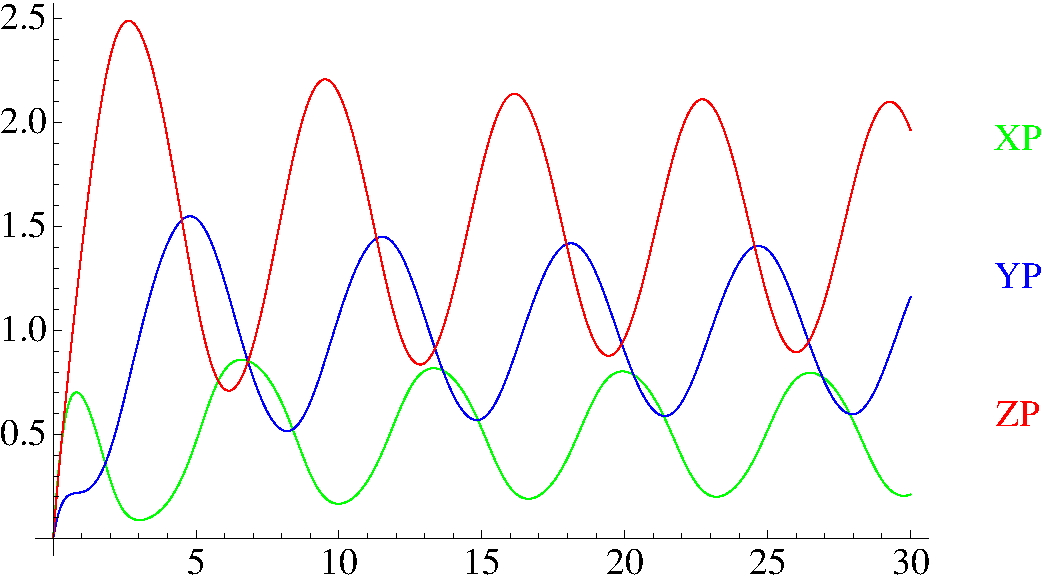
\includegraphics[scale=0.5]{ring-oscillator.pdf}
\end{center}
  
To save the model to a CelleratorML file {\ttfamily RingOscillator.xml} we use the command:
\begin{verbatim}
SaveModel[
 "RingOscillator.xml", 
  reactions, 
 "Name" -> Ring, 
 "Parameters" -> someRateConstants, 
 "InitialConditions" -> someInitialConditions, 
 "Descrioption" -> 
  "Ring Oscillator based on Michaelis Menten Kinetics"]
\end{verbatim}  
We can retrieve the model from the XML with:

\begin{verbatim}
{m, p, ics,  opts} = GetModel["RingOscillator.xml"]
\end{verbatim}

and then run the same simluation on the retrieved model with

\begin{verbatim}
run[m, timeSpan -> 30, initialConditions -> ics, 
 rates -> p, plot -> True, plotVariables -> {XP, YP, ZP}]
 \end{verbatim}

\subsubsection{Coupled Ring Oscillators}

We now consider a system of coupled oscillators as described in the previous section. We define a template of
ten random ``cells'' by

\begin{verbatim}
   n = 10; 
   r := RandomReal[{0, 100}]; 
   centers = Table[{r, r}, {n}];
\end{verbatim}

We couple the reactions by allowing the species X, Y, and Z to diffuse with rates DX, DY, and DZ. 
We would normally generate the Cellzilla model with

\begin{verbatim}
   sys = GenerateSystem[
     centers, 
     reactions, 
     {{X, DX}, {Y, DY}, {Z, DZ}}, 
     {i, j}];
\end{verbatim}

For initial conditions, we start X, Y, Z with random values between 0 and 3, and XP, YP, and ZP at zero:

\begin{verbatim}
   icOnTemplate = {
      X -> Table[RandomReal[{0, 3}], {n}], 
      Y -> Table[RandomReal[{0, 3}], {n}], 
      Z -> Table[RandomReal[{0, 3}], {n}], 
      XP -> Table[0, {n}], 
      YP -> Table[0, {n}], 
      ZP -> Table[0, {n}]};
   icOnTemplate = ListICToCellzillaIC[icOnTemplate];
\end{verbatim}

Here {\ttfamily ListToCellzillaIC} is a function in CelleratorML.m that converts initial conditions from 
a list of numbers to the format required by cellzilla.\\

We can then run a simulation and plot each of the variables {\ttfamily XP[1], XP[2], ..., XP[10]} with

\begin{verbatim}
   runPlot[sim, XP /@ Range[n]]
\end{verbatim}

A typical plot showing the convergence towards synchronized oscillations is illustrated below: 
\begin{center}
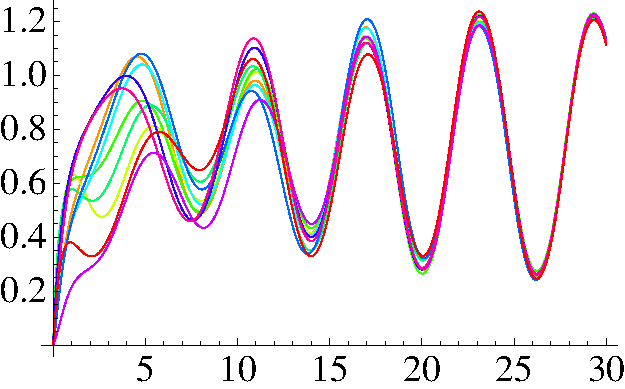
\includegraphics[scale=0.7]{ringsync.pdf}
\end{center}


To save the Cellzilla model to a CellzillaML file {\ttfamily Multiple-Ring-Oscillators.xml} we use:

\begin{verbatim}
  SaveCellzillaModel["Multiple-Ring-OScillators.xml", 
   "Models" -> {"RingOscillator.xml"},
   "Centers" -> centers,
   "Parameters" -> {DX -> 1, DY -> 1, DZ -> 1}, 
   "InitialConditions" -> icOnTemplate, 
   "DiffusingSpecies" -> {{X, DX}, {Y, DY}, {Z, DZ}}
   ] 
\end{verbatim}

The CellzillaML file contains all of the information necessary to reproduce the model: a reference to
a stand-alone cellerator model in {\ttfamily RingOscillator.xml}; a list of cell centers; additional parameters
that are not defined in the stand-alone model; the initial conditions; and the diffusing species. Note that we 
do not have to re-specify the parameter values if we want to re-use the ones that are in {\ttfamily RingOscillator.xml}. If we
had respecified any of the parameters, on reloading the model, any parameter values in the CellzillaML file take precedence
over the parameter values in the CelleratorML file. 

To recover the model and reproduce the simulations, we use the function {\ttfamily GetCellzillaModel} as follows: 

\begin{verbatim}
  czm = GetCellzillaModel["Multiple-Ring-OScillators.xml"];
  
  ckt2 = GenerateSystem[
   "Centers" /. czm,
   "Circuit" /. czm,
   "DiffusingSpecies" /. czm, 
   {i, j}];
   
  sim2 = run[
     ckt2, {0, 30},
     rates -> "Parameters" /. czm,
     initialConditions -> ListICToCellzillaIC["IC" /. czm]
     ];

\end{verbatim}

Note that in the {\ttfamily run} command we have to wrap the initial conditions with {\ttfamily ListToCellzillaIC} because {\ttfamily GetCellzillaModel} returns the initial conditions in the form {\ttfamily \{X->\{value, value, ..\}, Y->\{value, value, ..\}, ..\}} whereas Cellzilla requires them in the form {\ttfamily \{X[1]-> value, X[2]->value, ...\}}. The reason for this discrepency is for future SME and Cambium compatibility.

 

  
\subsection{Function Reference}
\subsubsection*{CellzillaICToList}
\begin{verbatim}
CellzillaICToList}[
  {a[1]->val, a[2]->val,.., b[1]->val, b[2]->val, ..}]
\end{verbatim}
returns a list
\begin{verbatim}
  {a->{val,val,..}, b->{val, val,..}, ..}
\end{verbatim}

\subsubsection*{GetCellzillaModel}
{\ttfamily GetCellzillaModel[filename, options]}\\

imports a CellzillaML file and returns the following data structure as a list of options (may be in any order):

\begin{verbatim}
{"Circuit"->list of cellerator reactions
"Parameters"->{name->value, name->value,..}
"IC"->{name->{val,val,val,..}, name->{val, val, val,..}, ..}
"DiffusingSpecies"->{{species,rate}, {species, rate}, ..}
"Centers"->{{x1,y1}, {x2, y2},..}}
"Tissue"->Tissue[...]
\end{verbatim}

The Centers and Tissue objects will only be present if they exist in the xml file. It a Tissue object is present, there is no need for a Centers object, although it may be present. If the Tissue is missing, the Centers are required.\\

{\ttfamily GetCellzillaModel} has the following options: \\

{\ttfamily "Quiet"$\to$False};  If {\ttfamily True}, printing of messages during import will be suppressed.

\subsubsection*{GetModel}

{\ttfamily GetModel[filename, options]} returns the following list:
\begin{verbatim}
 {model, list-of-reation-rates, list-of-initial-conditions, list-of-options}
\end{verbatim}
where {\ttfamily list-of-options} is a list of the form 
\begin{verbatim} 
{"Name"->modelname, "Frozen"->{v1,v2,..}}. 
\end{verbatim}
where v1, v2, .. are Cellerator frozen variables. \\

{\ttfamily GetModel} has only one option:\\ 

{\ttfamily "Quiet"->False}, if {\ttfamily True}, will reduce the amount of printed output.

\subsubsection*{LatexForm}
{\ttfamily
LatexForm[model, rules, ic, outputfile.tex]
}
generates a latex file describing the model.\\

{\ttfamily LatexForm[model, rules, ic]} automatically generates an output file name.\\

In each of these forms, {\ttfamily model} is a list of cellerator reactions; 
{\ttfamily rules} is a list of cellerator rate rules; and {\ttfamily ic} is a list of cellerator initial condition rules.\\

{\ttfamily LatexForm[inputfile.xml, outputfile.tex]} converts the CelleratorML file to latex.\\

{\ttfamily LatexForm[inputfile.xml]} autogenerates an output file name.\\

In any case if the specified output file already exists, a unique new file name is generated.\\

The return value of {\ttfamily LatexForm} is always the name of the file created, or {\ttfamily \$Failed} if it was unable to create a file.

\subsubsection*{ListICToCellzillaIC}

\begin{verbatim} 
ListICToCellzillaIC[
  {a->{val1,val2,..}, 
  b->{val1,val2,..},..}]\end{verbatim}
 returns a list 
 \begin{verbatim}
 {a[1]->val, a[2]->val,.., b[1]->val, b[2]->val, ..}
 \end{verbatim}
 
\subsubsection*{SaveCellzillaModel}
\begin{verbatim}
SaveCellzillaModel[filename,
	"Models"->{file1,file2,URL3,...}
	"Centers"->{{x1,y1},{x2,y2},..}
	"Tissue"->Tissue[...]
	"Parameters"->{sym->value,sym->value,..}
	"InitialConditions"{A[1]->value,A[2]->value,..., Z[n]->value}
	"DiffusingSpecies"->{{species,rate}, {species, rate}, ..}
	]
\end{verbatim}

Either a Cellzilla2D Tissue object or a list of Centers is required.\\



If {\ttfamily filename} is omitted, the model is written to the current notebook.


\subsubsection*{SaveModel}

{\ttfamily SaveModel[model, options]} writes a Cellerator model into xml text to screen.\\

{\ttfamily SaveModel[filename, model, options]} writes xml to specified file; If the file already exists it is not overwritten, but a new file with a unique file name is created.\\

Options (note that all options are quoted strings, not symbols):\\

{\ttfamily "Name"}$\to$Optional model name.\\
{\ttfamily	"Parameters"}$\to$Optional list of parameters  (equivalent to SME reactionRates or run option rates).\\
{\ttfamily	"InitialConditions"}$\to$Optional list of initial conditions (equivalent to SME initialCondi or run option initialConditions).\\
{\ttfamily	"Frozen"}$\to$\{\}, List of Cellerator frozen varibles.\\
{\ttfamily	"email"}$\to$Optional creator's email for annotation.\\
{\ttfamily	"WebPage"}$\to$Optional creator's web page for annotation.\\
{\ttfamily	"Description"}$\to$Optional text or html description of model for annotation.\\

Example:

\begin{verbatim}
SaveModel[
  {{A->B, k1}, {B->Q, k2}}, 
  "Parameters"->{k1->1, k2->2}, 
  "InitialConditions"->{A->5, B->7, Q->0}]
\end{verbatim}


\end{document}